\documentclass[12pt, a4paper]{article}
\usepackage{amsthm,amsfonts,amsmath,amssymb,amscd}
\usepackage[T2A]{fontenc}                         
\usepackage[utf8]{inputenc}                      
\usepackage[english, russian]{babel}
\usepackage{graphicx}
\usepackage{indentfirst}
\usepackage{multicol}
\usepackage{titlesec}
\usepackage{url}
\usepackage[hidelinks]{hyperref}
%\usepackage{cite} 
%\usepackage{psfrag}
%\IfFileExists{pscyr.sty}{\usepackage{pscyr}}{}    %

\usepackage[top=2cm,bottom=2cm,left=1.5cm,right=1.5cm]{geometry}

\titleformat{\section}
  {\normalfont\fontsize{12}{15}\bfseries}{\thesection}{1em}{}
  
\titleformat{\subsection}
  {\normalfont\fontsize{12}{14}\bfseries}{\thesubsection}{1em}{}
  
\titleformat{\subsubsection}
  {\normalfont\fontsize{12}{12}\bfseries}{\thesubsubsection}{1em}{}
 
\begin{document}
\begin{center}
Отчет о проделанной работе от 30.08.2022\\

\textbf{<<Разработка комбинированной математической модели распространения COVID-19 с учетом экономических агентов>>}\\
Воробьева Ирина
\end{center}

Для моделирования влияния пандемии COVID-19 на экономику предлагается взять за основу модели межотраслевого баланса. На основе данной модели предлагается изучать распространение шоков в экономике. В качестве основного шока предлагается рассматривать влияние пандемии Covid-19 на занятость и трудоспособность населения.

\section{Построение матрицы межотраслевого баланса для Новосибирской области}
\subsection{Используемые данные}
Использование методов анализа межотраслевого баланса предполагает наличие соответствующей матрицы. Матрицы межотраслевого баланса в Российской Федерации строятся только на национальном уровне, поэтому при моделировании экономики отдельно взятого региона необходимо перейти от национальных матриц межотраслевого баланса к региональным.

В первую очередь нужно определить, на основе каких статистических данных строится модель межотраслевого баланса. Симметричная таблица Затрат-Выпусков строится раз в 5 лет, наиболее актуальной является таблица за 2016 год \cite{RosstatZV}. Однако, в работах \cite{AkimovaCourse}, \cite{PonomEvdok} при анализе используются таблицы использования товаров и услуг, которые Росстат предоставляет ежегодно. В работе \cite{AkimovaCourse} строится матрица норм затрат, усредненная за период с 2012 по 2019 год, однако в рассматриваемой задаче о влиянии пандемии на экономику региона будут рассматриваться таблицы за предшествующий пандемии 2019 год  \cite{RosstatTRI}.

Таблица использования отечественной продукции в основных ценах содержит информацию о том, каким образом выпуски отраслей распределяются по произведенной продукции. Другой важной информацией в таблице являются данные об импорте, экспорте товаров и услуг и валовой добавленной стоимости. Необходимо проверять соответствие продукции, представленной в таблице, выделенным отраслям. Сделать это можно с помощью сравнения кодов ОКВЭД и ОКПД \cite{OKPD}.
 Всего в таблице выделены 61 отрасль и 61 вид товаров.

Алгоритмы локализации матриц межотраслевого баланса для регионального уровня описаны в \cite{Flegg}, а в работе \cite{PonomEvdok} применены для регионов Российской Федерации по таблице использования товаров и услуг за 2017 год. В работе \cite{Kronenberg} 
 проведены исследования, позволяющие выбрать наиболее подходящий метод построения коэффициентов локализации. Для применения методов локализации используются данные о занятости населения в различных отраслях экономики как внутри рассматриваемого для локализации региона, так на национальном уровне. Такие данные ежегодно собирает и предоставляет Росстат \cite{RegionStat}. 
 Среди представленной информации есть данные о численности рабочей силы по годам и о распределении среднегодовой численности занятых по видам экономической деятельности за различные годы (до 2020).

Для уточнения полученных с помощью метода локализации результатов воспользуемся данными об отраслевой структуре валовой добавленной стоимости в рассматриваемом регионе и данными о ВДС по регионам внутри страны. Такие данные также ежегодно (с задержкой на 2 года) публикуются Росстатом \cite{RegionStat}.

В результате получены все необходимые данные для построения таблицы метожраслевого баланса для любого из регионов РФ. Далее, в качестве примера, будем рассматривать Новосибирскую область. По собранным данным аналогичные преобразования и построения можно провести для любого субъекта Федерации или федерального округа.

\subsubsection{Обработка данных}

В описанных ранее таблицах по-разному выбраны отрасли, для которых происходит агрегирование значений. Для таблицы использования товаров и услуг выделяется 61 отрасль, в таблице с распределением занятых выделено всего групп 14 отраслей. Таким образом, необходимо построить таблицу соответствия отраслей из разных таблиц и провести агрегирование по отраслям. Для группировки будем использовать оператор агрегирования $T = \{t_{ij}\}_{i = 1, \ldots, m}^{j = 1, \ldots, n}$, где $n$ --- число отраслей до агрегации, $m$ --- число отраслей в матрице после агрегации. Если мы хотим, чтобы после действия оператора $j$-я отрасль попала в $i$-ю, то $t_{ij} = 1$, если нет, то $t_{ij} = 0$. В таком случае, для матрицы технологических коэффициентов $A = \{a_{ij}\}_{i, j = 1, \ldots, n}$ агрегированная матрица $\bar{A}$ получается по формуле $\bar{A} = T A T^T.$ Также необходимо помнить о группировке значений внутри векторов использования продукции и первичных ресурсов в соответствующих отраслях. В приложении представлена таблица соотношения между отраслями из таблицы о распределении среднегодовой численности занятых по видам экономической деятельности и таблицы использования товаров и услуг, таблица, группирующая товары по соответствующим им отраслям, а также полученная в результате агрегирования отраслей усеченная таблица использования товаров и услуг для Российской Федерации за 2019 год. В этой таблице содержатся данные о межотраслевом взаимодействии 14 выделенных групп отраслей, совокупные данные об использовании продукции, а также данные о первичных ресурсах: валовая добавленная стоимость, в которую входит, в том числе, и оплата труда, и остальные объединенные внутри групп отраслей первичные ресурсы.

Для построения коэффициентов локализации строится отношение численности трудящихся в отрасли в выбранном регионе к численности трудящихся в этой отрасли на национальном уровне. Для того, чтобы сравнивать эти величины, объединим данные из двух рассматриваемых таблиц, связанных с занятостью населения. В первой таблице <<Рабочая сила>> содержатся данные о численности рабочей силы в регионе, во второй таблице <<Распределение среднегодовой численности занятых по видам экономической деятельности>> результаты представлены в процентах внутри региона. Для того, чтобы получить искомые данные умножим каждую строку второй таблицы (данные о распределении по отраслям внутри региона) на совокупную численность занятых внутри региона из первой таблицы.
Для данных о ВДС регионов проводим аналогичные действия и получаем ВДС по отраслям внутри региона в денежном выражении.

В результате, были получены таблицы межотраслевого баланса для РФ за 2019 год по группам отраслей, соответствующих данным о занятости населения. Имеющиеся данные позволяют построить локальную матрицу межотраслевого баланса для Новосибирской области.

\subsection{Построение матрицы локализации}

Для построения коэффициентов локализации воспользуемся алгоритмом из 
\cite{PonomEvdok}. 
В рассматриваемом методе элементы регионального межотраслевого баланса $z_{ij}^R$ получаются из произведения регионального отраслевого выпуска $x_j^R$ и регионального технологического коэффициента $a_{ij}^R$: $$z^R_{ij} = a^R_{ij} x_j^R$$. 

Из предположения о схожей структуре производства одного продукта в различных регионах, можно получить формулу для определения $x_{j}^R$ из национального отраслевого выпуска:
$$
x_j^R = \dfrac{L_j^R}{L_j^N}x_j^N,
$$
где $L_j^R,\ L_j^N$ --- региональная и национальная занятость в отрасли $j$. Данные о национальном отраслевом выпуске содержатся в таблице использования товаров и услуг, региональная и национальная занятость является суммой по строкам в построенной ранее таблице.

Технологический коэффициент можно интерпретировать как количество единиц региональной продукции $i$ для производства единицы региональной продукции $j$. 
Коэффициент локализации $a_{ij}^R$ строится путем нормировки национальных коэффициентов: 
$$a_{ij}^R = \left\{ \begin{aligned}&t_{ij}a_{ij}^N,\quad t_{ij} \leqslant 1,\\&a_{ij}^N,\quad t_{ij} > 1\end{aligned}\right.$$. 

Коэффициент $t_{ij}$ отвечает за локализацию. Существуют различные подходы к его построению, далее будем рассматривать коэффициент FLQ, который, согласно статьям, 
\cite{Kronenberg}, \cite{Bonfiglio} 
дает наиболее точные результаты. Такой метод расчета коэффициента локализации позволяет учитывать как межотраслевую структуру занятости в регионе, так и размер региона.

Введем следующие обозначения: $L^R$ --- общая занятость в регионе, $L^N$ --- общая занятость на национальном уровне, $L_i^R,\ L_i^N$ --- общая занятость в $i$-й отрасли на региональном и национальном уровне соответственно, $\delta \geqslant 1$ --- эндогенный параметр. При таких обозначениях искомый коэффициент $t_{ij}$ равен
$$
t_{ij} = \mathrm{FLQ}_{ij} = \left\{\begin{aligned}
& \dfrac{L_i^R L_j^N}{L_i^N L_j^R}\lambda,\quad i \neq j,\\
& \dfrac{L_i^R l^N}{L^R L_i^N}\lambda,\quad i=j,
\end{aligned}\right.
$$
где $\lambda = \left[\log_2\left(1 + \dfrac{L^R}{L^N}\right)\right]^\delta$, $\delta \in [0, 1]$. Множитель $\lambda$ позволяет
\cite{RassShan} учитывать размер региона внутри страны, а параметр $\delta$ в его определении выбирается таким образом, чтобы получить наиболее согласованные с реальными данными результатами. Параметр $\delta$ выбирался таким образом, чтобы суммарный выпуск отраслей не превышал разницу между ожидаемым совокупным выпуском и валовой добавленной стоимостью, полученной из статистических данных.

Таблица для Новосибирска за 2019 год, полученная описанным образом, приведена в приложении.

\section{Моделирование воздействия шоков на экономику Новосибирской области}
\subsection{Описание модели с учетом имеющихся данных}
В основе выбранного метода для исследования экономики Новосибирской области лежит модель межотраслевого баланса, так как именно моделирование межотраслевых связей позволяет изучать комплектное влияние шоков, в том числе в отдельных отраслях, на экономику рассматриваемой системы. Первые работы по решению задачи построения модели межотраслевого баланса написаны А.В.Леонтьевым \cite{Leontief}. В его модели считается, что связь между отраслями можно описать с помощью матрицы технологических коэффициентов: они описывают потребность $i$-й отрасли в продукции $j$-й отрасли. Считается, что произведенная продукция расходуется на следующий производственный цикл и на потребление. Обозначим потребление через $Z = (Z_1, \ldots, Z_n)$, а выпуск через $Y = (Y_1, \ldots, Y_n)$. Матрицу технологических коэффициентов обозначим через $A = \{a_{ij}\}_{i,j = 1, \ldots, n}$, причем $a_{ij} \geqslant 0$ для любых $i, j$. В таком случае, сформулированную ранее гипотезу о распределении произведенной продукции можно записать следующим образом:
$$
Z = (E - A)Y,
$$
где $E$ --- единичная матрица.

Рассмотрим систему из $m$ отраслей. Введем вектор $X^j = (X^j_1, \ldots, X^j_m)$, где $X_i^j$ --- объем продукции $i$-й отрасли, необходимый для производства в $j$-й отрасли. Будем также предполагать, что в процессе производства каждая из отраслей использует первичные ресурсы, обозначим это через $l^j = (j_1^j, \ldots, l_n^j)$. Для каждой отрасли введем производственные функции, $F_j(X^j, l^j)$, будем считать, что они обладают неоклассическими свойствами (вогнуты, монотонно неубывают, непрерывны и обращаются в нуле в нуль).

Через $X^0 = (X^0_1,\ldots, X^0_m)$ обозначим объемы поставок производимой продукции отраслями, а $F_0(X^0)$ --- функция полезности репрезентативного потребителя.

Рассмотрим задачу об оптимальном использовании первичных ресурсов, ограниченных вектором $(l_1, \ldots, l_n)$, в целях максимизации функции полезности потребителя \cite{RassShan}, \cite{AkimovaCourse}. Запишем данную задачу в виде задачи выпуклого программирования \eqref{syst1}.

\begin{equation}\label{syst1}
\begin{aligned}
&F_0(X^0) \rightarrow \max;\\
&F_j(X^j, l^j) \geq \sum\limits_{i=0}^{m}X_j^i, j = 1,\ldots,m;\\
&\sum\limits_{j=1}^m l^j \leq l;\\
&X^0 \geq 0, \ldots, X^m \geq 0, l^1 \geq 0,\ldots,l^n \geq 0. 
\end{aligned}
\end{equation}

Далее через $Z = \{Z_i^j\}_{i=1,\ldots m+n}^{j = 1, \ldots, m+k}$ будем обозначать усеченную таблицу использования товаров и услуг. Число рассматриваемых отраслей $m = 14$, все потребители собраны в одного $k = 1$, а в качестве первичных ресурсов рассматриваются ВДС и Импорта $n = 2$.

По таблице использования товаров и услуг построим:
\begin{itemize}
\item $Z^0 = (Z_1^0, \ldots, Z_m^0)$, где $Z_i^0 = \sum\limits_{j = m + 1}^{m + k}$. В рассматриваемой нами таблице $k = 1$ (все конечные потребители объединены в одного), поэтому в рассматриваемом случае $Z^0$ - последний столбец матрицы использования товаров и услуг;
\item $A_0 = \sum\limits_{i=1}^m Z_i^0$ --- совокупное конечное потребление;
\item $A_j = \sum\limits_{i=1}^{m+n} Z_i^j$ --- совокупные средства производства, необходимые $j$-й отрасли;
\item $a_{ij} = Z_i^j / A_j$ --- технологические коэффициенты;
\item $b_{ij} = Z_{m+i}^j / A_j$ --- доля первичных ресурсов в производственных средствах $j$-й отрасли;
\item $a^0_i = Z_i^0 / A_0$ --- доля потребления, покрытая $i$-й отраслью.
\end{itemize}

В работе 
\cite{RassShan} 
показано, что набор значений переменных из таблицы межотраслевого баланса 
$$
\left\{
\begin{aligned}
&\hat{X}_i^0 = Z_i^0,\quad i = 1,\ldots, m,\\
&\hat{X}_i^j = Z_i^j,\quad i = 1,\ldots m, j=1,\ldots,m,\\
&\hat{l}_t^j = Z_{m+t}^j, \quad t = 1, \ldots, n, j = 1,\ldots, m
\end{aligned}
\right\}
$$
является решением задачи выпуклого программирования \eqref{syst1}.

Для задачи выпуклого программирования \eqref{syst1} можно построить двойственную задачу с сопряженными переменными $p = (p_1, \ldots, p_m)$ и $s = (s_1, \ldots, s_n)$, которые интерпретируются как цены на продукцию, производимую отраслями, и цены на первичные ресурсы соответственно. Двойственная задача имеет вид \eqref{syst2}.

\begin{equation}\label{syst2}
\begin{aligned}
&(\hat{X}^j, \hat{l}^j) \in \text{Argmax}\left\{p_jF_j(X^j, l^j) - p X^j - sl^j \Biggl|X^j \geq 0, l^j \geq 0\right\},\quad j = 1,\ldots, m;\\
&p_j\left[F_j(\hat{X}^j, \hat{l}^j) - \hat{X}^0 - \sum\limits_{i=1}^{m}\hat{X}^i_j\right] = 0;\quad j=1,\ldots, m\\
&s_k\left[l_k - \sum\limits_{j=1}^m \hat{l}^j_k\right] = 0,\quad k = 1,\ldots,n;\\
&\hat{X}^0 \in \text{Argmax}\left\{p_0F_0(X^0) - pX^0\right\}.
\end{aligned}
\end{equation}

Будем рассматривать производственные функции вида Кобба--Дугласа:
$$
F_j(X^j, l^j) = \alpha_j (X1^j)^{a_{1i}}\cdot \ldots \cdot (X_m^j)^{a_{mj}}(l_1^j)^{b_{1j}}\cdot \ldots \cdot (l_n^j)^{b_{nj}}, \quad j = 1, \ldots, m.
$$

В качестве функции полезности потребителей также рассмотрим функцию Кобба--Дугласа вида 
$$
F_0(X^0) = (X^0_1)^{a_1^0}\cdot \ldots \cdot (X_m^0)^{a^0_m}.
$$

При таком выборе функций полезности и производственных функций в работе 
\cite{RassShan} 
показано, что решением двойственной задачи для цен на продукцию отраслей при некоторых фиксированных ценах на первичные ресурсы является вектор $p = (p_1, \ldots, p_m)$, c
$$
p_j = e^{\mu_j} s_1^{c_{ij}}\cdots \ldots \cdot s_n^{c_{nj}},
$$
где\begin{itemize}
\item $C = \{c_ij\}_{i = 1,\ldots,n}^{j = 1, \ldots, m} = (E - A^T)^{-1}B^T,$ 
\item $d = (\ln(F_1(a_1, b_1)), \ldots, \ln F_m(a_m, b_m))^T,$
\item $\mu = -(E - A^T)^{-1}d$.
\end{itemize} 

В таком случае, ВВП (валовой внутренний продукт) рассматриваемой экономики можно записать следующим образом:
\begin{equation}\label{GDP}
GDP = \dfrac{A_0}{F_0(a_0)}e^{-(\mu_1a^0_{1}+\ldots+\mu_m a^0_m)}.
\end{equation}

Таким образом, мы знаем, что экономическая система находится в равновесии, и что наблюдаемые статистически значения матрицы межотраслевого баланса являются оптимальными по распределению первичных ресурсов с целью максимизации ВВП. Однако, в моменты воздействия шоков на экономику система выходит из положения равновесия. Анализ влияния шоков помогает показать, каким образом неоптимальное поведение сказывается на функции полезности потребителей, а через нее и на ВВП. 

\subsection{Описание введения шоков в экономику}
В предложенной задаче рассматривается распространение шоков, вызванное изменениями выпусков отраслей: во время пандемии многие предприятия вынуждены были приостановить работу, значительная часть сотрудников также не могла выполнять свои обязанности в связи с болезнью, в результате чего объем производимой продукции уменьшился. Рассмотрим, каким образом изменения выпуска в отдельных отраслях (более или менее подверженных воздействиям пандемии) оказывают влияние на экономику рассматриваемых экономических систем.

В основе описанной ранее модели лежит гипотеза постоянства коэффициентов прямых затрат в межотраслевом взаимодействии, которую можно описать следующим образом:
\begin{equation}\label{Leontev}
Y = AY + Z,
\end{equation}
где $Y$ --- вектор выпуска товаров, $Z$ - вектор потребления товаров, а $A = \{a_{ij}\}$ --- матрица технологических коэффициентов прямых затрат. 

При изменении выпусков изменяется величина $Y$, которая, при выполнении гипотезы о сохранении технологических коэффициентов, оказывает влияние на конечное потребление $X_0 = Z$. В результате, через объемы конечного потребления оказывается влияние на формирование значения ВВП рассматриваемой экономики по формуле \eqref{GDP}.
Сравнение значений ВВП до и после внесения шоков могут отражать силу изменений, вызванных воздействием шоков, в частности пандемии Covid-19, в рассматриваемой экономике.

\subsection{Описание численного моделирования}

Главным параметром, изменение которого рассматривается при моделировании является относительное изменение ВВП. В описанной ранее модели нет четкой привязки в текущему ВВП, тем более, что на региональном уровне в статистике принято выделять значение ВРП (валовой региональный продукт), которое по сути является валовой добавленной стоимостью, а не валовым внутренним продуктом. Полученные в результате моделирования значения ВВП региона сравниваются со значениями, полученными при моделировании оптимального случая (без внесения изменений в выпуск), а результат выражается в процентах от ВВП при оптимальных значениях параметров.

В первую очередь, при моделировании из матрицы использования товаров и услуг строятся коэффициенты, описанные ранее: $A_0,\ A_j,\ a_{ij},\ b_{ij}$ и прочие. На их основе строятся производственные функции и функция полезности вида Кобба--Дугласа с коэффициентами 
$$\alpha_j = A_j \prod\limits_{i=1}^{m} \dfrac{1}{(Z_i^j)^{a_{ij}}}\prod\limits_{i=1}^{n}\dfrac{1}{(Z_{m+i}^j)^{b_{ij}}},\quad \alpha_0 = A_0 \prod\limits_{i=1}^m\dfrac{1}{(Z_i^0)^{a_i^0}}.$$
Таким образом были построены функции полезности для оптимальных финансовых потоков и использования начальных запасов.

Для моделирования падения выпуска будем уменьшать оптимальные значения выпуска на 10\%, 15\%, 20\%. Затем, пользуясь матрицей технологических коэффициентов восстановим значения конечного использования продукции. Подставляя значения в описанную ранее функцию для определения ВВП и нормируя полученный результат на ВВП до внесения каких-либо изменений, получим искомую величину.
\section{Результаты численного моделирования}
В данном разделе представлены результаты моделирования воздействия шоков на различные отрасли экономики Новосибирской области. Рассматриваются следующие сценарии:
\begin{enumerate}
\item падение выпуска во всех отраслях экономики;
\item падение выпуска в трех наиболее значимых, с точки зрения ВДС, отраслях экономики;
\item падение выпуска в трех наиболее важных, с точки зрения численности занятых, отраслях.
\end{enumerate}
\subsection{Падение выпуска во всех отраслях}

Падение выпуска во всех отраслях не приводит к существенным изменениям в межотраслевом взаимодействии, так как падение одинаково для всех рассматриваемых отраслей. В этом случае относительный ВВП уменьшается пропорционально уменьшению выпусков.

Таким образом, при уменьшении выпуска на 10\%, 15\% и 20\% получим следующие результаты:
\begin{center}
\begin{tabular}{|c|c|}
\hline
Падение выпуска & Относительное изменение ВВП (\%) \\
\hline
0\% & 100\% \\
10\% &94,7\% \\
15\% & 89,5\% \\
20\% & 84,2\%\\
\hline
\end{tabular}
\end{center}

Также результаты представлены на рис.\ref{fig1}.

\begin{figure}[h]
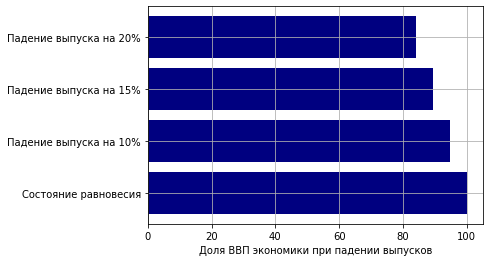
\includegraphics[width=0.8\textwidth]{pictures/shock1.png}\label{fig1}
\caption{Изменение выпуска во всех отраслях}
\end{figure}
\subsection{Падение выпуска в главных отраслях}

Рассмотрим распределения ВДС и распределение рабочей силы по отраслям. Заметим, что в обоих случаях доминирующие отрасли (за исключением <<Других видов деятельности>>) совпадают. Эти отрасли:
\begin{enumerate}
\item транспортировка и хранение;
\item торговля оптовая и розничная;
\item обрабатывающие производства.
\end{enumerate}
Заметим, что порядки, в которых эти отрасли убывают, отличаются для двух рассматриваемых критериев. 


\begin{figure}[h]
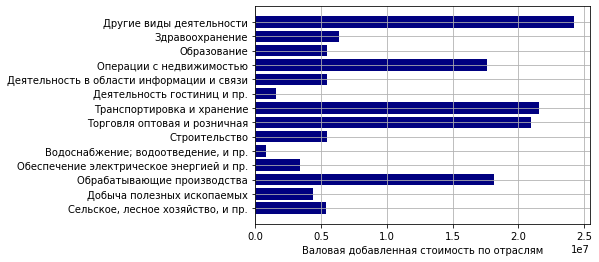
\includegraphics[width=0.9\textwidth]{pictures/VDS.png}
\caption{Валовая добавленная стоимость в Новосибирской области}
\end{figure}

\begin{figure}[h]
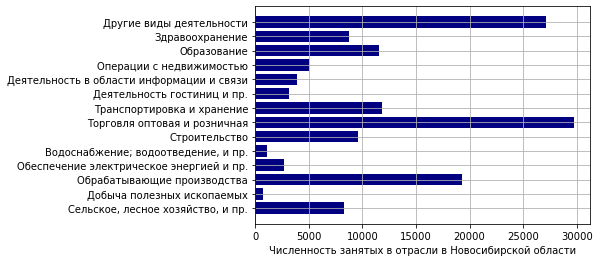
\includegraphics[width=0.9\textwidth]{pictures/labour.png}
\caption{Занятость населения в Новосибирской области}
\end{figure}
Рассмотрим несколько вариантов изменения выпуска: изменение выпуска в отдельно выбранной отрасли из трех и изменение выпуска во всех отраслях одновременно. Это позволит выделить наиболее важную, с точки зрения влияния на ВВП экономики, отрасль и оценить относительное изменение ВВП при изменениях во всех выбранных отраслях.

Влияние падения выпуска в трех главных отраслях представлено в следующей таблице.

\begin{figure}[h]
\begin{tabular}{|c|c|c|c|}
\hline
Изменение выпуска & Обрабатывающие производства & Торговля & Транспортировка\\
\hline
0\% & 100\% & 100\% & 100\%\\
10\% & 97,5\% &98,5\% & 99,1\%\\
15\% & 96,1\%& 97,7\%& 98,5\%\\
20\% & 94,5\%& 96,8\%& 98\%\\
\hline
\end{tabular}

\end{figure}

Из полученных результатов можно сделать вывод о том, что изменения в отрасли <<Обрабатывающие производства>> являются наиболее значимыми из рассматриваемых отраслей.

При внесении изменения во все отрасли одновременно получаются следующие результаты.
\begin{center}
\begin{tabular}{|c|c|}
\hline
Падение выпуска & Относительное изменение ВВП\\
\hline
0\% & 100\%\\
10\% & 95,2\%\\
15\% & 92,7\%\\
20\% & 90,7\\
\hline
\end{tabular}
\end{center}

Получается, что уменьшение выпусков в трех отраслях одновременно приводит к более значительным изменениям ВВП, причем падение ВВП примерно равно половине от падения ВВП при уменьшении выпуска во всех отраслях экономики региона одновременно. Таким образом, выбранные отрасли являются центральными для экономики Новосибирской области.

\section{Влияние пандемии на экономику Новосибирской области}

Влияние пандемии Covid-19 можно исследовать с использованием двух различных подходов. Первый подход <<снизу-вверх>> предполагает, что изменения на уровне численности трудящихся оказывают существенное влияние на выпуски в экономике. Второй подход <<сверху-вниз>> подразумевает использование локализованных данных о изменениях в экономике Российской Федерации. Далее рассмотрим оба подхода и сравним полученные результаты.

\subsection{Влияние пандемии на рынок труда в регионе}
По данным региональной статистики о занятости населения \cite{RegionStat}  можно исследовать изменение численности трудящихся в отдельных отраслях региона. На Рис.\ref{labour} показано относительное изменение численности трудящихся в отраслях по отношению к 2015 году. Представлена лишь часть отраслей, которые либо оказывают наиболее существенное влияние на экономику региона (обрабатывающие производства, торговля оптовая и розничная, транспортировка и хранение, образование), либо наиболее подвержены влиянию  пандемии Covid-19 (здравоохранение, деятельность гостиниц и пр.).
\begin{figure}[h]
\center
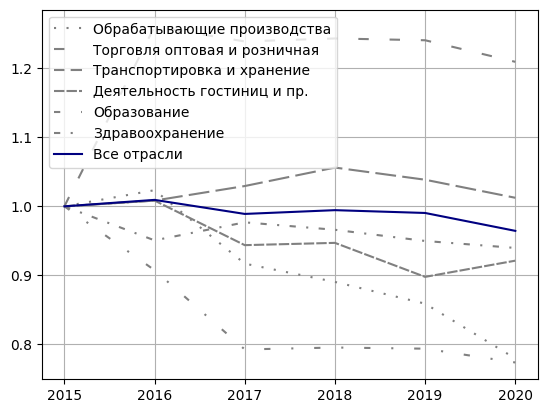
\includegraphics[width=0.7\textwidth]{pictures/labour_branches.png}\
\caption{Динамика численности трудящихся в Новосибирской области}
\label{labour}
\end{figure}

На графике видно, что данный показатель не является устойчивым во времени, поэтому сравнивать изменения относительно только 2019 года не корректно. В качестве оценки силы шока в отдельной отрасли предлагается рассматривать экспоненциально сглаженное среднее значение числа занятых за период с 2015 по 2019 годы. Такой подход позволяет учитывать как  тренд изменения числа трудящихся в отдельных отраслях, так и нестабильность части показателей: для них изменения, связанные с пандемией могут быть не так заметны. В таблице на Рис. \ref{t_labour} представлены усредненные значения численности трудящихся по отраслям внутри региона.
 
\begin{figure}[h]
\begin{center}
\begin{tabular}{|l|l|}
\hline
Отрасль & Средняя занятость (тыч. чел.) \\
\hline
 Сельское, лесное хозяйство и пр &  78.04\\
 Добыча полезных ископаемых & 34.76 \\
 Обрабатывающие производства & 192.14\\
 Обеспечение электрической энергией и пр. &  39.48 \\
 Водоснабжение, водоотведение и пр. & 12.69 \\
 Строительство &  98.70 \\
 Торговля оптовая и розничная & 259.41 \\
Транспортировка и хранение & 109.66 \\
 Деятельность гостиниц и пр. & 44.83 \\
 Деятельность в области информации и связи & 29.15 \\
 Операции с недвижимостью & 31.93\\
 Образование & 148.60 \\
 Здравоохранение & 94.74\\
 Другие виды деятельности & 261.39\\
\hline
\end{tabular}
\label{t_labour}
\caption{Численность трудящихся в Новосибирской области, усредненная с 2015 по 2019 годы}
\end{center}
\end{figure}

Получив эту величину, можно оценить величину шоков, вызванных изменением численности работников в различных отраслях как отношение численности трудящихся в отраслях в 2020 году к усредненным за прошлые годы значениям. Размеры таких шоков изображены на Рис.~\ref{labour_shock}. Однако, не всегда можно предполагать, что численность сотрудников напрямую оказывает влияние на выпуск отраслей. 

\begin{figure}[h]
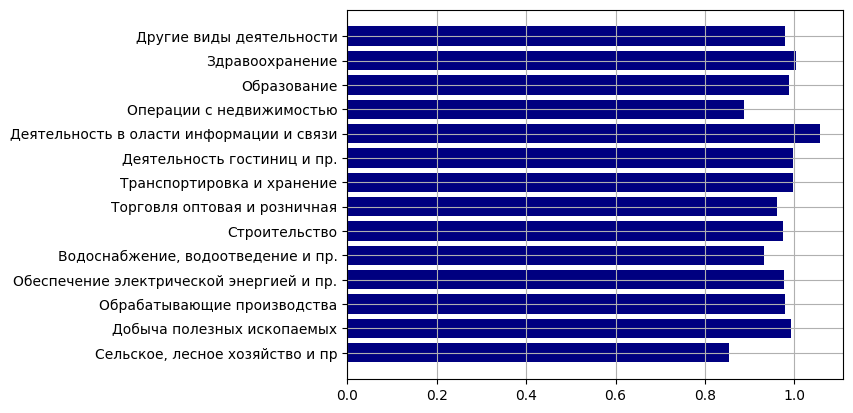
\includegraphics[width=0.9\textwidth]{pictures/labour_shock.png}
\caption{Шоки по численности трудящихся}
\label{labour_shock}
\end{figure}

\subsection{Оценка изменений выпусков в регионе}
На момент написания работы нельзя напрямую оценить изменение ВРП Новосибирской области в 2020 году по отношению к доковидному 2019 году, так как нет статистических данных об отраслевой структуре ВРП. Однако, существует отраслевая структура ВВП РФ за 2020 год, локализация которой может позволить оценить масштаб изменений выпусков в различных отраслях в выбранном регионе. На Рис. \ref{vvp_rf} представлена остраслевая структура ВВП РФ в 2019 и 2020 годах.

\begin{figure}[h]
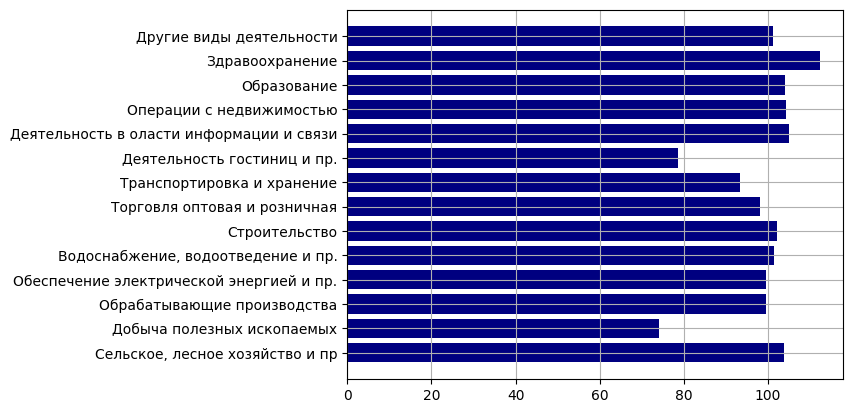
\includegraphics[width=0.9\textwidth]{pictures/vvp_rf.png}
\caption{Отношение показателя ВВП РФ в отрасли в 2020 году к 2019 году}
\label{vvp_rf}
\end{figure}

Для оценки изменения отраслевой структуры выпусков в Новосибирской области между 2019 и 2020 годом проведем локализацию шоков на национальном уровне. Будем считать, что если отрасль в регионе развита также, как и на национальном уровне, то и шоки будут схожими. Таким образом, чтобы определить шок в отрасли внутри некоторого региона, нам необходимо домножить национальный шок на мультипликатор $\alpha_j$, характеризующий важность данной отрасли в выбранном регионе. В качестве такого мультипликатора будем использовать отношение доли трудящихся в выбранной отрасли на региональном и национальных уровнях:
$$
\alpha_j = \dfrac{L_j^R}{L^R} \cdot \dfrac{L^N}{L_j^N}.
$$
\begin{figure}
\begin{center}
\begin{tabular}{|l|l|l|}
\hline
Отрасль & Новосибирская область & Российская Федерация\\
\hline
 Сельское, лесное хозяйство и пр &  0.058 & 0.066\\
 Добыча полезных ископаемых & 0.005  &  0.015\\
 Обрабатывающие производства & 0.135 &  0.139\\
 Обеспечение электрической энергией и пр. &  0.019 & 0.022\\
 Водоснабжение, водоотведение и пр. & 0.008  & 0.009\\
 Строительство &  0.067  & 0.089\\
 Торговля оптовая и розничная &  0.208 & 0.189\\
Транспортировка и хранение & 0.083 &  0.075\\
 Деятельность гостиниц и пр. & 0.022 & 0.024\\
 Деятельность в области информации и связи & 0.027 & 0.021\\
 Операции с недвижимостью &  0.035 & 0.026\\
 Образование & 0.081 &0.075 \\
 Здравоохранение & 0.061 &  0.061\\
 Другие виды деятельности & 0.190 &0.177\\
\hline
\end{tabular}
\label{t_lab_vvp}
\caption{Соотношение трудящихся в отрасли к трудящимся в регионе}
\end{center}
\end{figure}

В таком случае, для Новосибирской области могут быть получены следующие размеры шоков в 2020 году (Рис. \ref{vvp_novosib}). На полученной диаграмме видно, что шоки в менее развитых областях значительно уменьшаются на региональном уровне, по сравнению с национальным (пример --- добыча полезных ископаемых).
Наиболее сильно пострадавшими отраслями являются отрасли, связанные с путешествиями и перевозками, а также торговлей. Заметим, что в приведенном ранее анализе экономики региона торговля и транспорт оказывали сильное влияние на экономическую ситуацию.
\begin{figure}
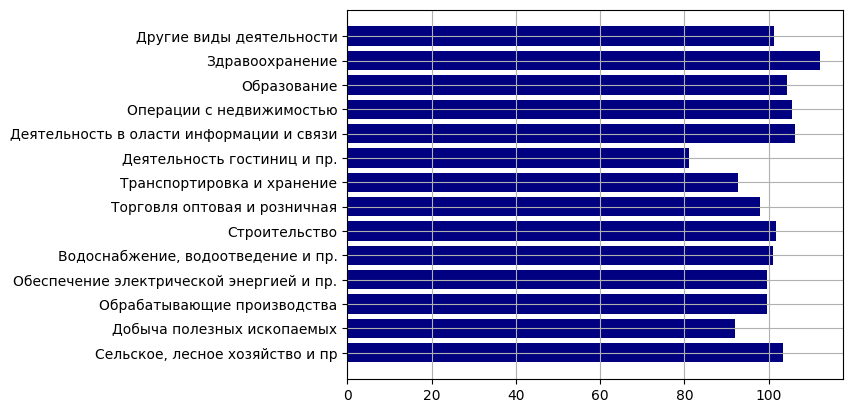
\includegraphics[width=0.9\textwidth]{pictures/vvp_novosib.png}\
\caption{Шоки по выпускам в отраслях.}
\label{vvp_novosib}
\end{figure}


\subsection{Сравнительный анализ влияния шоков на экономику региона}

В таблице \ref{shock_compare} представлены величины шоков, полученные двумя различными способами. Видно, что значения могут отличаться. Это связано с предположением о том, что изменения в численности трудящихся в некоторой отрасли напрямую оказывают влияние на размер выпуска. Также при таком подходе не удается оценить влияние изменений в объемах спроса на выбранные группы товаров. Во втором подходе недостатком является его синтетичность: на текущий момент не существует статистических данных, позволяющих оценить изменения напрямую на региональном уровне, поэтому приходится прибегать к коэффициентам локализации, что также может вызывать неточности в результатах. В Новосибирской области шоки по наиболее значимым отраслям экономики: транспорт, торговля, обрабатывающие производства упали одинаково в обоих подходах.


\begin{figure}
\begin{center}
\begin{tabular}{|l|l|l|}
\hline
 Отрасль & Шоки (численность) & Шоки (выпуски)\\
\hline
 Сельское, лесное хозяйство и пр &  0.85 & 1.03\\
 Добыча полезных ископаемых & 0.99 & 0.91\\
 Обрабатывающие производства & 0.97 & 0.99\\
 Обеспечение электрической энергией и пр. &  0.97 & 0.99\\
 Водоснабжение, водоотведение и пр. & 0.93 & 1.01\\
 Строительство &  0.97 & 1.01\\
 Торговля оптовая и розничная & 0.96 & 0.97\\
 Транспортировка и хранение & 0.99 & 0.92\\
 Деятельность гостиниц и пр. & 0.99 & 0.81\\
 Деятельность в области информации и связи & 1.05 & 1.06\\
 Операции с недвижимостью & 0.88 & 1.05\\
 Образование & 0.98 & 1.04\\
 Здравоохранение & 1.00 & 1.12\\
 Другие виды деятельности & 0.97 & 1.01\\
\hline
\end{tabular}
\label{shock_compare}
\caption{Сравнение величины шоков, полученных с использованием двух разных подходов}
\end{center}
\end{figure}

Применим полученные значения шоков к рассматриваемой ранее модели и сравним результаты, полученные с использованием альтернативных подходов.

\begin{center}
\begin{tabular}{|c|c|}
\hline
Воздействие шоков & Относительное изменение ВВП\\
\hline
Нет шоков & 100\%\\
Подход 1 & 99,1\%\\
Подход 2 & 96,7\%\\
\hline
\end{tabular}
\end{center}

Ни в одном из случаев оцененные шоки не привели к относительному росту ВВП, наоборот,  шоки, вызванные пандемией, привели к спаду в экономике. 

В первом подходе, опирающемся исключительно на изменения в численности трудящихся, относительный ВВП упал менее, чем на 1\%. Такой результат позволяет говорить, что пандемия не оказала существенного влияния на ситуацию на рынке труда. Принимаемые меры позволили поддержать здоровье граждан, привели к тому, что в сжатые сроки люди смогли вернуться к работе.

Во втором подходе учитываются комплексные изменения, вызванные пандемией. Например видно, как она повлияла на добычу полезных ископаемых: спрос на них по миру упал, что привело к сильным изменениям в выпусках, хотя численность трудящихся в данной отрасли изменилась слабо. В результате, сильный спад в отраслях, связанных со сферой услуг, падение в ключевых отраслях региональной экономики и добыче полезных ископаемых пересилили влияние роста секторов здравоохранения, недвижимости, деятельности в области информации и связи.
\section{Заключение}
В рамках данной работы была построена экономическая модель Новосибирской области, опирающаяся на модель межотраслевого баланса. Построенные коэффициенты локализации позволили обойти ограниченность статистики в сфере таблиц <<Затраты-Выпуски>> на региональном уровне и построить модель межотраслевого взаимодействия внутри выбранного региона.

Для изучения влияния пандемии на экономику региона была использована модель учета шоков в экономике: описано, каким образом изменения в выпусках оказывают влияние на состояние экономики системы в целом. В результате, это позволило выделить наиболее важные для региона отрасли экономики, рассмотреть их влияние на состояние региона в целом.

Ключевой задачей была оценка влияния пандемии: необходимо определить силу влияния Covid-19 на отдельные отрасли в экономике. Для этого было использовано два подхода: подход <<снизу-вверх>>, в котором было сделано предположение о том, что численность трудящихся в отдельной отрасли оказывает серьезное влияние на ее выпуск. В данном подходе не учитываются экзогенные факторы экономики, такие как изменения спроса.
Второй подход <<сверху-вниз>> представляет собой локализацию изменений в экономике на государственном уровне. В этом случае учитываются внешние, но не внутренние изменения: ключевым фактором, осуществляющим локализацию, является соотношение труда на региональном и национальном уровнях.
В результате, в обоих случаях отмечается спад в экономике, причем комплексные факторы приводят к более значительному снижению относительного ВВП. 
\newpage
\bibliography{resource.bib}
\bibliographystyle{plain}

%\bibitem{Inverse_Shan}
%Россоха~А.~В., Шананин~А.~А, <<Обратные задачи анализа межотраслевых балансов>>, Матем. моделирование, 33:3 (2021), 39 -- 58.
%\bibitem{Duality_Shan}
%Шананин~А.~А. Двойственность по Янгу и агрегирование балансов // Доклады РАН. Математика, информатика, процессы управления, 2020, т.493, с.81-85.
%\bibitem{Akimova}
%Акимова~Е.~Д. Выпускная квалицикационная работа <<Сетевые модели экономического роста>>, Москва, 2021.
%\bibitem{Akimova_course}
%Акимова~Е.~Д. Курсовая работа <<Использование межотраслевого баланса для решения современных проблем межотраслевых связей>>, Москва, 2022.
%\bibitem{Leontev}
%Леонтьев~В.~В. Экономические эссе. -- М.: Политиздат, 1990, 404 с.
%\bibitem{COVID_model}
% Криворотько О.И., Кабанихин С.И., Сосновская М.И., Андорная Д.В. Анализ чувствительности и идентифицируемости математических моделей распространения эпидемии COVID-19. Вавиловский журнал генетики и селекции, \textbf{25}(1), 82--91 (2021).
%\bibitem{COVID_code}
%COVID-19 Agent-based Simulator \underline{https://github.com/InstituteforDiseaseModeling/covasim}

%\bibitem{Region_stat}
%Регионы России. Социально-экономические показатели - 2021 год \underline{https://gks.ru/bgd/regl/b21\_14p/Main.htm}
%\bibitem{Rosstat_stat}
%Росстат, таблицы <<затраты-выпуск>> --- 2016 год \underline{https://rosstat.gov.ru/statistics/accounts}
%\bibitem{Rosstat_TRI}
%Таблицы ресурсов и использования товаров и услуг Российской Федерации за 2019 год \underline{https://rosstat.gov.ru/storage/mediabank/tri-2019.xlsx}

%\bibitem{MOB_stat1}
%Коган~А.~Б., <<Межотраслевой анализ экономики Новосибирской области>>, Вестник НГУЭУ, 2015.
%\bibitem{MOB_stat2}
%Котова~Т.~Е. <<Оценка внешнеторговых эффектов в экономике Хабаровского
%края на основе использования таблиц «затраты–выпуск» >> Пространственная
%экономика. 2012. No 1. С. 43–68.
%\bibitem{MOB_Flegg}
%A.~T.~Flegg , C.~D.~Webber \& M.~V.~Elliott (1995) On the Appropriate Use of Location Quotients in Generating Regional Input–Output Tables, Regional Studies, 29:6, 547-561, DOI:~10.1080/00343409512331349173
%\bibitem{MOB_Accur}
%Kronenberg~T. <<Regional input-output models and the treatment of imports in the European System of Accounts (ESA)>> Jahrbuch für Regionalwissenschaft. 2012. Vol. 32. Рр. 175-191.
%\bibitem{MOB_Monte_Carlo}
%Bonfiglio~A. <<On the Parameterization of Techniques for Representing Regional Economic Structures>> Economic System Research. 2009. Vol. 212. Pp. 115-127.
%\bibitem{MOB_loc_base}
%Пономарев~Ю.~Ю., Евдокимов~Д.~Ю., <<Построение усеченных таблиц <<Затраты-Выпуск>> для регионов России с использованием коэффициентов локализации>>, Проблемы прогнозирования, 2021, No 6.
%\bibitem{OKVED}
%Расшифровка кодов ОКВЭД и их классификация \underline{https://xn----dtbec0aczc1l.xn--p1ai/\#1}
%\bibitem{OKPD}
%Общероссийские экономические классификаторы, закрепленные за минэкономразвития России \underline{https://www.economy.gov.ru/material/departments/d18/obshcherossiyskie\_klassifikatory\_zakreplennye\_za\_minekonomrazvitiya\_rossii/}.

\newpage
\section{Приложения}
\subsection{Соотношение отраслей таблицы распределения занятых по отраслям и отраслей из таблицы использования товаров и услуг}

Далее: 
\begin{itemize}\item таблица 1 --- таблица распределения среднегодовой численности занятых по видам деятельности, \item таблица 2 --- таблица использования товаров и услуг в основных ценах.\end{itemize}

\begin{tabular}[t]{|c|p{6cm}|p{9cm}|}
\hline
	№ & Таблица 1 & Таблица 2\\
\hline
1 & Сельское, лесное хозяйство, охота, рыболовство и рыбоводство &  
 Растениеводство и животноводство, охота и предоставление соответствующих услуг в этих областях\\\cline{3-3}
 && Лесоводство и лесозаготовки\\ \cline{3-3}
 && Рыболовство и рыбоводство\\\cline{1-3}
2 & Добыча полезных ископаемых & Добыча полезных ископаемых\\\cline{1-3}
3 & Обрабатывающие производства & Производство пищевых  продуктов,  напитков, табачных изделий \\\cline{3-3}
&&Производство пищевых  продуктов,  напитков, табачных изделий  \\ \cline{3-3}
&& Обработка древесины и производство изделий из дерева и пробки, кроме мебели, производство изделий из соломки и материалов для плетения  \\ \cline{3-3}
&& Производство бумаги и бумажных изделий \\ \cline{3-3}
&& Деятельность полиграфическая и копирование носителей информации \\ \cline{3-3}
&& Производство кокса и нефтепродуктов \\ \cline{3-3}
&& Производство химических веществ и химических продуктов \\ \cline{3-3}
&& Производство лекарственных средств и материалов, применяемых в медицинских целях \\ \cline{3-3}
&& Производство резиновых и пластмассовых изделий \\ \cline{3-3}
&& Производство прочей неметаллической минеральной продукции \\ \cline{3-3}
&& Производство металлургическое \\ \cline{3-3}
&& Производство готовых металлических изделий, кроме машин и оборудования \\ \cline{3-3}
&& Производство компьютеров, электронных и оптических изделий \\ \cline{3-3}
&& Производство электрического оборудования \\ \cline{3-3}
&& Производство машин и оборудования, не включенных в другие группировки \\ \cline{3-3}
&& Производство автотранспортных средств, прицепов и полуприцепов \\ \cline{3-3}
&& Производство прочих транспортных средств и оборудования \\ \cline{3-3}
&& Производство мебели, прочих готовых изделий \\ \cline{3-3}
&& Ремонт и монтаж машин и оборудования \\ \cline{1-3}

\end{tabular}

\begin{tabular}[t]{|c|p{6cm}|p{9cm}|}
\hline
	№ & Таблица 1 & Таблица 2\\
\hline
4 & Обеспечение электрическое энергией, газом и паром; кондиционирование воздуха & Обеспечение электрической энергией, газом и паром; кондиционирование воздуха\\ \cline{1-3}
5 & Водоснабжение; водоотведение, организация сбора и утилизации отходов, деятельность по ликвидации загрязнений & Забор, очистка и распределение воды\\ \cline{3-3}
&& Сбор и обработка сточных вод; сбор, обработка и утилизация отходов; обработка вторичного сырья; предоставление услуг в области ликвидации последствий загрязнений и прочих услуг, связанных с удалением отходов \\ \cline{1-3}
6 & Строительство & Строительство\\ \cline{1-3}
7 & Торговля оптовая и розничная; ремонт автотранспортных средств и мотоциклов & Торговля оптовая и розничная автотранспортными средствами и мотоциклами и их ремонт\\ \cline{3-3}
&& Торговля оптовая,  кроме оптовой торговли автотранспортными средствами и мотоциклами \\ \cline{3-3}
&& Торговля розничная, кроме торговли автотранспортными средствами и мотоциклами \\ \cline{1-3}
8 & Транспортировка и хранение & Деятельность сухопутного и трубопроводного транспорта\\ \cline{3-3}
&& Деятельность водного транспорта \\ \cline{3-3}
&& Деятельность воздушного и космического транспорта\\ \cline{3-3}
&& Складское хозяйство и вспомогательная транспортная деятельность \\ \cline{3-3}
&& Деятельность почтовой связи и курьерская деятельность \\ \cline{1-3}
9 & Деятельность гостиниц и предприятий общественного питания & Деятельность гостиниц и предприятий общественного питания\\ \cline{1-3}
10 & Деятельность в области информации и связи & Деятельность издательская\\ \cline{3-3}
&& Производство кинофильмов, видеофильмов и телевизионных программ, издание звукозаписей и нот; деятельность в области телевизионного и радиовещания \\ \cline{3-3}
&& Деятельность в сфере телекоммуникаций \\ \cline{3-3}
&& Разработка компьютерного программного обеспечения, консультационные услуги в данной области и другие сопутствующие услуги; деятельность в области информационных технологий \\ \cline{1-3}
11 & Деятельность по операциям с недвижимым имуществом & Деятельность по операциям с недвижимым имуществом\\ \cline{1-3}
12 & Образование & Образование\\ \cline{1-3}
\end{tabular}


\begin{tabular}[t]{|c|p{6cm}|p{9cm}|}
\hline
	№ & Таблица 1 & Таблица 2\\
\hline
13 & Деятельность в области здравоохранения и социальных услуг & Деятельность в области здравоохранения \\ \cline{3-3}
&& Деятельность по уходу с обеспечением проживания; предоставление социальных услуг без обеспечения проживания \\ \cline{1-3}
14 & Другие виды деятельности & Деятельность финансовая и страховая\\ \cline{3-3}
&& Деятельность в области права и бухгалтерского учета; деятельность головных офисов; консультирование по вопросам управления \\ \cline{3-3}
&& Деятельность в области архитектуры и инженерно-технического проектирования; технических испытаний, исследований и анализа \\ \cline{3-3}
&&Научные исследования и разработки \\ \cline{3-3}
&& Деятельность рекламная и исследование конъюнктуры рынка \\ \cline{3-3}
&& Деятельность профессиональная научная и техническая прочая; деятельность ветеринарная  \\ \cline{3-3}
&& Аренда и лизинг \\ \cline{3-3}
&& Деятельность по трудоустройству и подбору персонала \\ \cline{3-3}
&& Деятельность туристических агентств и прочих организаций, предоставляющих услуги в сфере туризма \\ \cline{3-3}
&& Деятельность по обеспечению безопасности и  проведению расследований, обслуживанию зданий и территорий, административно-хозяйственная, вспомогательная деятельность по обеспечению функционирования организации, деятельность по предоставлению прочих вспомогательных услуг для бизнеса \\ \cline{3-3}
&& Государственное управление и обеспечение военной безопасности; социальное обеспечение \\ \cline{3-3}
&& Деятельность творческая, в области искусства и организации развлечений, библиотек, архивов, музеев и прочих объектов культуры, по организации и проведению азартных игр и заключению пари, по организации и проведению лотерей \\ \cline{3-3}
&& Деятельность в области спорта, отдыха и развлечений \\ \cline{3-3}
&& Деятельность общественных организаций \\ \cline{3-3}
&& Ремонт компьютеров, предметов личного потребления и хозяйственно-бытового назначения \\ \cline{3-3}
&& Деятельность по предоставлению прочих персональных услуг \\ \cline{1-3}

\end{tabular}

\subsection{Соотношение отраслей таблицы распределения занятых по отраслям и продукции из таблицы использования товаров и услуг}

Далее: 
\begin{itemize}\item таблица 1 --- таблица распределения среднегодовой численности занятых по видам деятельности, \item таблица 2 --- таблица использования товаров и услуг в основных ценах.\end{itemize}

\begin{tabular}[t]{|c|p{6cm}|p{9cm}|}
\hline
	№ & Таблица 1 & Таблица 2\\
\hline
1 & Сельское, лесное хозяйство, охота, рыболовство и рыбоводство &  
 Продукция и услуги сельского хозяйства и охоты\\\cline{3-3}
 && Продукция лесоводства, лесозаготовок и связанные с этим услуги\\ \cline{3-3}
 && Рыба и прочая продукция рыболовства и рыбоводства; услуги, связанные с рыболовством и рыбоводством\\\cline{1-3}
2 & Добыча полезных ископаемых & Продукция горнодобывающих производств\\\cline{1-3}
3 & Обрабатывающие производства & Продукты пищевые, напитки, изделия табачные \\\cline{3-3}
&&Текстиль и изделия текстильные, одежда, кожа и изделия из кожи  \\ \cline{3-3}
&& Древесина и изделия из дерева и пробки, кроме мебели; изделия из соломки и материалов для плетения  \\ \cline{3-3}
&&Бумага и изделия из бумаги \\ \cline{3-3}
&& Услуги печатные и услуги по копированию звуко- и видеозаписей, а также программных средств \\ \cline{3-3}
&&Кокс и нефтепродукты \\ \cline{3-3}
&& Вещества химические и продукты химические \\ \cline{3-3}
&&Средства лекарственные и материалы, применяемые в медицинских целях \\ \cline{3-3}
&& Изделия резиновые и пластмассовые \\ \cline{3-3}
&& Продукты минеральные неметаллические прочие \\ \cline{3-3}
&& Металлы основные \\ \cline{3-3}
&& Изделия металлические готовые, кроме машин и оборудования \\ \cline{3-3}
&& Оборудование компьютерное, электронное и оптическое \\ \cline{3-3}
&& Оборудование электрическое \\ \cline{3-3}
&& Машины и оборудование, не включенные в другие группировки \\ \cline{3-3}
&& Средства автотранспортные, прицепы и полуприцепы \\ \cline{3-3}
&& Средства транспортные и оборудование, прочие \\ \cline{3-3}
&& Мебель, изделия готовые прочие\\ \cline{3-3}
&& Услуги по ремонту и монтажу машин и оборудования \\ \cline{1-3}

\end{tabular}

\begin{tabular}[t]{|c|p{6cm}|p{9cm}|}
\hline
	№ & Таблица 1 & Таблица 2\\
\hline
4 & Обеспечение электрическое энергией, газом и паром; кондиционирование воздуха & Электроэнергия, газ, пар и кондиционирование воздуха\\ \cline{1-3}
5 & Водоснабжение; водоотведение, организация сбора и утилизации отходов, деятельность по ликвидации загрязнений & Вода природная; услуги по очистке воды и водоснабжению\\ \cline{3-3}
&& Услуги по водоотведению; шлам сточных вод; услуги по сбору, обработке и удалению отходов; услуги по утилизации отходов; услуги по рекультивации и прочие услуги по утилизации отходов \\ \cline{1-3}
6 & Строительство & Сооружения и строительные работы\\ \cline{1-3}
7 & Торговля оптовая и розничная; ремонт автотранспортных средств и мотоциклов & Услуги по оптовой и розничной торговле и услуги по ремонту автотранспортных средств и мотоциклов\\ \cline{3-3}
&& Услуги по оптовой торговле, кроме оптовой торговли автотранспортными средствами и мотоциклами \\ \cline{3-3}
&& Услуги по розничной торговле, кроме розничной торговли автотранспортными средствами и мотоциклами \\ \cline{1-3}
8 & Транспортировка и хранение & Услуги сухопутного и трубопроводного транспорта\\ \cline{3-3}
&& Услуги водного транспорта \\ \cline{3-3}
&&Услуги воздушного и космического транспорта\\ \cline{3-3}
&&Услуги по складированию и вспомогательные транспортные услуги \\ \cline{3-3}
&& Услуги почтовой связи и услуги курьерские\\ \cline{1-3}
9 & Деятельность гостиниц и предприятий общественного питания & Услуги гостиничного хозяйства и общественного питания\\ \cline{1-3}
10 & Деятельность в области информации и связи & Услуги издательские\\ \cline{3-3}
&& Услуги по производству кинофильмов, видеофильмов и телевизионных программ, звукозаписей и изданию музыкальных записей; услуги в области теле- и радиовещания \\ \cline{3-3}
&& Услуги телекоммуникационные \\ \cline{3-3}
&& Продукты программные и услуги по разработке программного обеспечения; консультационные и аналогичные услуги в области информационных технологий; услуги в области информационных технологий \\ \cline{1-3}
11 & Деятельность по операциям с недвижимым имуществом & Услуги, связанные с недвижимым имуществом \\ \cline{1-3}
12 & Образование & Услуги в области образования\\ \cline{1-3}
\end{tabular}


\begin{tabular}[t]{|c|p{6cm}|p{9cm}|}
\hline
	№ & Таблица 1 & Таблица 2\\
\hline
13 & Деятельность в области здравоохранения и социальных услуг & Услуги в области здравоохранения\\ \cline{3-3}
&& Услуги по предоставлению ухода с обеспечением проживания; услуги социальные без обеспечения проживания \\ \cline{1-3}
14 & Другие виды деятельности & Услуги финансовые и страховые\\ \cline{3-3}
&& Услуги юридические и бухгалтерские; услуги головных офисов; услуги консультативные в области управления предприятием \\ \cline{3-3}
&& Услуги в области архитектуры и инженерно-технического проектирования, технических испытаний, исследований и анализа\\ \cline{3-3}
&&Услуги и работы, связанные с научными исследованиями и экспериментальными разработками \\ \cline{3-3}
&& Услуги рекламные и услуги по исследованию конъюнктуры рынка \\ \cline{3-3}
&& Услуги профессиональные, научные и технические, прочие; услуги ветеринарные \\ \cline{3-3}
&& Услуги по аренде и лизингу \\ \cline{3-3}
&& Услуги по трудоустройству и подбору персонала \\ \cline{3-3}
&& Услуги туристических агентств, туроператоров и прочие услуги по бронированию и сопутствующие им услуги \\ \cline{3-3}
&& Услуги по обеспечению безопасности и проведению расследований; услуги по обслуживанию зданий и территорий; услуги в области административного, хозяйственного и прочего вспомогательного обслуживания \\ \cline{3-3}
&& Услуги в сфере государственного управления и обеспечения военной безопасности; услуги по обязательному социальному обеспечению \\ \cline{3-3}
&&Услуги в области творчества, искусства и развлечений; услуги библиотек, архивов, музеев и прочие услуги в области культуры; услуги по организации и проведению азартных игр и заключению пари, лотерей \\ \cline{3-3}
&& Услуги, связанные со спортом, и услуги по организации развлечений и отдыха \\ \cline{3-3}
&& Услуги общественных организаций \\ \cline{3-3}
&& Услуги по ремонту компьютеров, предметов личного потребления и бытовых товаров \\ \cline{3-3}
&& Услуги персональные прочие \\ \cline{1-3}

\end{tabular}


\subsection{Усеченная таблица использования товаров и услуг для Российской Федерации за 2019 год}

\begin{tabular}{|l|rrrrrr}
\hline
 &          1 &           2 &           3 &          4 &         5 &          6  \\
\hline
1               &  1287390.0 &        92.0 &   2816002.0 &     3724.0 &      60.0 &    15028.0 \\
2               &     3398.0 &   1111753.0 &   5750397.0 &   882327.0 &    2799.0 &   174001.0 \\
3               &  1141376.0 &    883845.0 &  12487483.0 &   452105.0 &  262727.0 &  3317815.0\\
4               &   139192.0 &    389844.0 &   1514335.0 &  3194692.0 &   85950.0 &    78011.0 \\
5               &     5864.0 &     14228.0 &    446466.0 &    60468.0 &  173868.0 &    16128.0 \\
6               &    22575.0 &    285736.0 &    228397.0 &   117016.0 &   26828.0 &   368356.0 \\
7               &   292351.0 &    196230.0 &   3000262.0 &   744150.0 &   81356.0 &   774626.0\\
8               &   152337.0 &   1133614.0 &   2689110.0 &    77345.0 &   47154.0 &   332401.0\\
9               &     1156.0 &      8363.0 &     30813.0 &     5514.0 &     489.0 &    16976.0 \\
10              &     7009.0 &     29166.0 &    218228.0 &    50409.0 &    4149.0 &    38361.0\\
11              &    20740.0 &    353925.0 &    328211.0 &    85572.0 &   16705.0 &   111274.0\\
12              &      716.0 &      3949.0 &     13088.0 &     3749.0 &     376.0 &     3323.0 \\
13              &     1107.0 &      4519.0 &     10561.0 &     2868.0 &     654.0 &     2128.0 \\
14              &   216633.0 &    504233.0 &   1862500.0 &   306019.0 &   64265.0 &   892858.0 \\
ВДС             &  3869506.0 &  12622497.0 &  14215328.0 &  2564061.0 &  497082.0 &  5340644.0 \\
Остальное &   389767.0 &    367612.0 &   5754452.0 &   169053.0 &   90952.0 &  1073868.0 \\
\end{tabular}

\begin{tabular}{|l|rrrrrrrr|}
\hline
& 7 &          8 &         9 &         10 &         11 &         12 &      \\
\hline
1 & 8461.0 &     7443.0 &   48795.0 &       57.0 &      429.0 &     7908.0 \\
2 &   269490.0 &   126923.0 &     119.0 &       70.0 &     1227.0 &      558.0 \\
3&    655179.0 &  1859379.0 &  347323.0 &   214216.0 &   331331.0 &   111813.0\\
4&200326.0 &   416778.0 &   42645.0 &    56480.0 &   372180.0 &   162520.0 \\
5&32457.0 &    16220.0 &    6559.0 &     4783.0 &    87396.0 &    18571.0 \\
6&59543.0 &   187963.0 &   16997.0 &    12334.0 &   395515.0 &   163337.0\\
7&624948.0 &   448149.0 &   94369.0 &    64119.0 &   145224.0 &    36548.0 \\
8&3058146.0 &  2530136.0 &   21620.0 &    50255.0 &    23045.0 &    19529.0\\
9&22312.0 &    21206.0 &    4706.0 &     8771.0 &     1294.0 &    32813.0  \\
10&  248872.0 &   104385.0 &    9797.0 &  1105923.0 &    44833.0 &    55916.0\\
11&1869811.0 &   790852.0 &  182723.0 &   270876.0 &   935145.0 &    30485.0 \\
12&7814.0 &    15145.0 &     384.0 &     3203.0 &      691.0 &    58643.0 \\
13&6956.0 &     9347.0 &    1472.0 &     2116.0 &      512.0 &    15730.0 \\
14&1794620.0 &   969039.0 &  157293.0 &   381473.0 &   396653.0 &   109080.0 \\
ВДС&  12737849.0 &  6743364.0 &  919199.0 &  2607431.0 &  9633892.0 &  3279619.0 \\
Остальное& 769006.0 &   977487.0 &  145883.0 &   417072.0 &   243401.0 &   181547.0  \\
\end{tabular}

\begin{tabular}{|l|rrr|}
\hline
& 13 &          14 &  Использование \\
\hline
1 &  6325.0 &     55289.0 &    3294114.0 \\
2 &   885.0 &     16274.0 &    9569385.0 \\
3&   336824.0 &   1478755.0 &   27485462.0 \\
4&   86142.0 &    420239.0 &    1559738.0 \\
5&   15078.0 &    109211.0 &     348117.0 \\
6&  101280.0 &    740550.0 &    9829371.0 \\
7&  197920.0 &    579167.0 &   15086371.0 \\
8& 40736.0 &    740527.0 &    4307861.0 \\
9&   37719.0 &    197245.0 &    1610507.0 \\
10& 26550.0 &    934535.0 &    2321046.0 \\
11& 59276.0 &    713288.0 &    6843885.0 \\
12&  11403.0 &     55441.0 &    4106692.0 \\
13&   41911.0 &     99147.0 &    4432913.0 \\
14& 161831.0 &   3746455.0 &   24184606.0 \\
ВДС& 2981095.0 &  23456688.0 &         \\
Остальное&  526966.0 &   2404747.0 &         \\
\hline
\end{tabular}


\subsection{Усеченная матрица использования товаров и услуг для Новосибирской области за 2019 год}


\begin{tabular}{|l|lllllll}
\hline
{} & 1 & 2 & 3 & 4 & 5 & 6 & 7  \\
\hline
1 & 11888.5 & 0.545273 &  29979.7 &  39.6464 &                                  0.638771 &  159.991 & 90.0773  \\
2  &   13.0591 & 1337.88 & 22099.8 &  3390.94 &                                            10.7571 & 668.717 &  1035.7   \\
3                      &                                            13535.5 &                    5238.44 &                      143086 &                                            5361.49 &                                            3115.67 &        39345.8 &                                            7769.74 \\
4 &                                             1414.1 &                    2310.56 &                     15384.7 &                                            26865.2 &                                            873.197 &        792.542 &                                            2035.18  \\
5 &                                            57.6932 &                    84.3277 &                     4392.57 &                                            594.917 &                                            1371.23 &        158.676 &                                             319.33 \\
6 &                                            206.681 &                    1693.52 &                     2091.05 &                                            1071.32 &                                            245.619 &         2515.6 &                                            545.135 \\
7 &                                               3936 &                    1163.03 &                     40393.3 &                                            10018.7 &                                            1095.32 &          10429 &                                            9229.38 \\
8  &                                            2046.02 &                     6718.8 &                     36117.2 &                                            1038.81 &                                            633.321 &        4464.45 &                                            41073.7 \\
9 &                                            12.5107 &                    49.5665 &                      333.47 &                                            59.6747 &                                            5.29215 &        183.721 &                                            241.469 \\
10     &                                            110.826 &                    172.863 &                     3450.61 &                                            789.787 &                                             62.952 &        541.625 &                                            3935.15\\
11 &                                            330.639 &                    2097.67 &                     5232.37 &                                            1340.71 &                                            253.462 &        1571.09 &                                            29808.7  \\
12                              &                                             9.3848 &                    23.4053 &                     171.548 &                                            49.1391 &                                            4.92833 &        43.5554 &                                             102.42 \\
13 &                                            13.3945 &                    26.7836 &                     127.786 &                                            34.7023 &                                            7.91328 &        25.7484 &                                            84.1663 \\
14                          &                                             2843.8 &                    2988.53 &                     24449.5 &                                            4017.19 &                                            843.624 &        11720.8 &                                            23558.5  \\
ВДС                                                &                                            53549.3 &                      43685 &                      181786 &                                            33820.6 &                                            8455.15 &        54958.5 &                                             209970 \\
Остальное                                          &                                            34009.5 &                    38557.2 &                      430314 &                                              48114 &                                            3586.38 &        49697.4 &                                             134578 \\
\hline
\end{tabular}


\begin{tabular}{|l|llllllll|}
\hline
{} &  8 & 9 & 10 & 11 & 12 & 13 & 14 & Использование \\
\hline
1 &    79.2395 &                                             519.48 &                                  0.606832 &                                           4.56721 &        84.19 &                                            67.3371 &                  588.617 &       80473.8 \\
2   &                    487.788 &                                           0.457338 &                                  0.269023 &                                           4.71558 &      2.14449 &                                            3.40121 &                  62.5439 &       77029.9 \\
3 &                    22050.3 &                                            4118.89 &                                   2540.38 &                                           3929.24 &      1325.99 &                                            3994.38 &                  17536.5 &        666461 \\
4  &                     4234.2 &                                            433.246 &                                   573.801 &                                           3781.11 &       1651.1 &                                            875.148 &                  4269.36 &       71113.4 \\
5  &                    159.581 &                                             64.531 &                                   47.0577 &                                           859.849 &      182.712 &                                            148.346 &                  1074.48 &       11050.2 \\
6  &                    1720.86 &                                            155.613 &                                   112.922 &                                           3621.06 &       1495.4 &                                             927.25 &                  6779.96 &        154095 \\
7&                    6033.55 &                                            1270.51 &                                   863.251 &                                           1955.19 &      492.055 &                                            2664.65 &                  7797.48 &        367035 \\
8 &                    37186.2 &                                            290.376 &                                    674.97 &                                           309.515 &      262.292 &                                            547.121 &                  9945.95 &        174021 \\
9 &                      229.5 &                                            44.9083 &                                   94.9232 &                                           14.0042 &      355.115 &                                             408.21 &                  2134.66 &       29211.2 \\
10 &                    1650.53 &                                             154.91 &                                     22528 &                                           708.897 &       884.14 &                                            419.807 &                  14776.8 &       76594.4 \\
11  &                    12607.8 &                                            2912.98 &                                   4318.33 &                                           19364.1 &      485.994 &                                            944.983 &                  11371.3 &        217452 \\
12   &                     198.51 &                                            5.03319 &                                   41.9826 &                                           9.05712 &      820.859 &                                            149.462 &                   726.68 &       84252.4 \\
13  &                    113.097 &                                            17.8109 &                                   25.6032 &                                           6.19511 &       190.33 &                                            499.935 &                  1199.66 &       84059.4 \\
14    &                    12720.8 &                                            2064.83 &                                    5007.7 &                                           5206.97 &      1431.92 &                                             2124.4 &                  52601.4 &        572116 \\
ВДС  &                     215606 &                                            15501.1 &                                   54958.5 &                                            176149 &      54958.5 &                                            63413.6 &                   242381 &              \\
Остальное   &                    250.827 &                                            5823.57 &                                   34993.1 &                                           94168.8 &      21985.6 &                                            9244.49 &                   350450 &              \\
\hline
\end{tabular}

\end{document} 

